\documentclass[12pt]{article}
\usepackage[left=1cm, right=1cm, top=2cm,bottom=1.5cm]{geometry} 

\usepackage[parfill]{parskip}
\usepackage[utf8]{inputenc}
\usepackage[T2A]{fontenc}
\usepackage[russian]{babel}
\usepackage{enumitem}
\usepackage[normalem]{ulem}
\usepackage{amsfonts, amsmath, amsthm, amssymb, mathtools}
\usepackage{tabularx}
\usepackage{hhline}

\usepackage{accents}
\usepackage{fancyhdr}
\pagestyle{fancy}
\renewcommand{\headrulewidth}{1.5pt}
\renewcommand{\footrulewidth}{1pt}

\usepackage{graphicx}
\usepackage[figurename=Рис.]{caption}
\usepackage{subcaption}
\usepackage{float}

%%Наименование папки откуда забирать изображения
\graphicspath{ {./images/} }

%%Изменение формата для ввода доказательства
\renewcommand{\proofname}{$\square$  \nopunct}
\renewcommand\qedsymbol{$\blacksquare$}

%%Изменение отступа на таблицах
\addto\captionsrussian{%
	\renewcommand{\proofname}{$\square$ \nopunct}%
}
%% Римские цифры
\newcommand{\RN}[1]{%
	\textup{\uppercase\expandafter{\romannumeral#1}}%
}

%% Для удобства записи
\newcommand{\MR}{\mathbb{R}}
\newcommand{\MQ}{\mathbb{Q}}
\newcommand{\MN}{\mathbb{N}}
\newcommand{\MTB}{\mathbb{T}}
\newcommand{\MI}{\mathrm{I}}
\newcommand{\MJ}{\mathrm{J}}
\newcommand{\MH}{\mathrm{H}}
\newcommand{\MT}{\mathrm{T}}
\newcommand{\MU}{\mathcal{U}}
\newcommand{\MV}{\mathcal{V}}
\newcommand{\MW}{\mathcal{W}}
\newcommand{\VN}{\varnothing}
\newcommand{\VE}{\varepsilon}

\theoremstyle{definition}
\newtheorem{defn}{Опр:}
\newtheorem{rem}{Rm:}
\newtheorem{prop}{Утв.}
\newtheorem{exrc}{Упр.}
\newtheorem{lemma}{Лемма}
\newtheorem{theorem}{Теорема}
\newtheorem{corollary}{Следствие}

\newenvironment{cusdefn}[1]
{\renewcommand\thedefn{#1}\defn}
{\enddefn}

\DeclareRobustCommand{\divby}{%
	\mathrel{\text{\vbox{\baselineskip.65ex\lineskiplimit0pt\hbox{.}\hbox{.}\hbox{.}}}}%
}
%Короткий минус
\DeclareMathSymbol{\SMN}{\mathbin}{AMSa}{"39}
%Длинная шапка
\newcommand{\overbar}[1]{\mkern 1.5mu\overline{\mkern-1.5mu#1\mkern-1.5mu}\mkern 1.5mu}
%Функция знака
\DeclareMathOperator{\sgn}{sgn}

%Функция ранга
\DeclareMathOperator{\rk}{\text{rk}}

%Обозначение константы
\DeclareMathOperator{\const}{\text{const}}

%Интеграл в большом формате
\DeclareMathOperator{\dint}{\displaystyle\int}
\newcommand{\ddint}[2]{\displaystyle\int\limits_{#1}^{#2}}

\newcommand{\smallerrel}[1]{\mathrel{\mathpalette\smallerrelaux{#1}}}
\newcommand{\smallerrelaux}[2]{\raisebox{.1ex}{\scalebox{.75}{$#1#2$}}}

\newcommand{\smallin}{\smallerrel{\in}}
\newcommand{\smallnotin}{\smallerrel{\notin}}

\newcommand*{\medcap}{\mathbin{\scalebox{1.25}{\ensuremath{\cap}}}}%
\newcommand*{\medcup}{\mathbin{\scalebox{1.25}{\ensuremath{\cup}}}}%

\makeatletter
\newcommand{\vast}{\bBigg@{3.5}}
\newcommand{\Vast}{\bBigg@{5}}
\makeatother

%Скалярное произведение
\DeclarePairedDelimiterX{\inner}[2]{\langle}{\rangle}{#1, #2}

%Подпись символов снизу
\newcommand{\ubar}[1]{\underaccent{\bar}{#1}}

%% Шапка для букв сверху
\newcommand{\wte}[1]{\widetilde{#1}}

\begin{document}
	\lhead{Математический анализ - \RN{2}}
	\chead{Шапошников С.В.}
	\rhead{Лекция - 24}
\section*{Суммы и интегралы Дарбу}
Всегда предполагаем, что $f$ - ограничена на изучаемом отрезке $[a,b]$.
\begin{defn}
	$\forall$ разбиения $\MTB$ отрезка $[a,b]$ следующая сумма:
	$$
		s(f,\MTB) = \sum\limits_{k = 1}^N \inf\limits_{\Delta_k}f{\cdot}|\Delta_k| 
	$$
	называется \uwave{нижней суммой Дарбу}.
\end{defn}

\begin{defn}
	$\forall$ разбиения $\MTB$ отрезка $[a,b]$ следующая сумма:
	$$
		S(f,\MTB) = \sum\limits_{k = 1}^N \sup\limits_{\Delta_k}f{\cdot}|\Delta_k| 
	$$
	называется \uwave{верхней суммой Дарбу}.
\end{defn}
\begin{lemma}
	Верны следующие утверждения:
	\begin{enumerate}[label={(\arabic*)}]
		\item $s(f,\MTB) = \inf\limits_{\xi}\sigma(f,\MTB,\xi) \leq \sigma(f,\MTB,\xi) \leq \sup\limits_{\xi}\sigma(f,\MTB,\xi) = S(f,\MTB)$;
		\item Пусть $\MTB \subset \MTB^\prime$ (измельчение разбиения $\MTB$), тогда $s(f,\MTB) \leq s(f,\MTB^\prime)$ и $S(f,\MTB) \geq S(f,\MTB^\prime)$;
		\item $\forall \, \MTB_1, \MTB_2, \, s(f,\MTB_1) \leq S(f,\MTB_2)$;
	\end{enumerate}
\end{lemma}

\begin{defn}
	Точная верхняя грань нижней суммы Дарбу:
	$$
		\underline{\MI} = \sup\limits_{\MTB}s(f,\MTB) 
	$$
	называется \uwave{нижним интегралом Дарбу}.
\end{defn}
\begin{defn}
	Точная нижняя грань верхней суммы Дарбу:
	$$
		\overline{\MI} = \inf\limits_{\MTB}S(f,\MTB) 
	$$
	называется \uwave{верхним интегралом Дарбу}.
\end{defn}

\begin{lemma}
	Нижний и верхний интегралы Дарбу можно определить следующим образом:
	$$
		\lim\limits_{\lambda(\MTB) \to 0}s(f,\MTB)  = \underline{\MI}, \, \lim\limits_{\lambda(\MTB) \to 0}S(f,\MTB)  =\overline{\MI}
	$$
\end{lemma}
\begin{proof}
	Рассмотрим первое равенство, предел мы понимаем в следующем смысле:
	$$
		\forall \VE > 0, \, \exists \, \delta > 0 \colon \forall \, \MTB, \, \lambda(\MTB) < \delta \Rightarrow \underline{\MI} - s(f,\MTB) < \VE
	$$
	По определению, нижний интеграл Дарбу это точная верхняя грань нижней суммы Дарбу, тогда:
	$$
		\forall \VE > 0, \, \exists \, \MTB_\VE \colon \underline{\MI} - \VE < s(f,\MTB_\VE)
	$$
	Пусть $\MTB$ - произвольное разбиение отрезка $[a,b]$. Рассмотрим следующую разность:
	$$
		\underline{\MI} - s(f,\MTB) = \underline{\MI} - s(f,\MTB_\VE) + s(f,\MTB_\VE) - s(f,\MTB) < \VE + s(f,\MTB_\VE) - s(f,\MTB)
	$$
	Возьмем $\MTB \cup \MTB_\VE$ - измельчение $\MTB_\VE$ и $\MTB$, тогда по предыдущей лемме:
	$$
		\VE + s(f,\MTB_\VE) - s(f,\MTB) \leq \VE + s(f,\MTB \cup \MTB_\VE) - s(f,\MTB)
	$$
	Пусть $\MTB$ разбивает отрезок $[a,b]$ на $\Delta_k$, а $\MTB \cup \MTB_\VE$ разбивает отрезок $[a,b]$ на $\Delta_m^\prime$. Среди отрезков $\MTB \cup \MTB_\VE$ есть те же самые, что и среди отрезков $\MTB$.
	\begin{figure}[H]
		\centering
		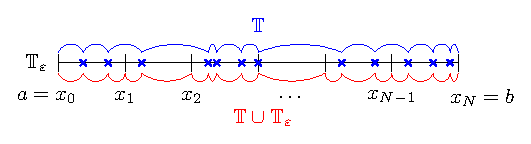
\includegraphics[width=0.7\textwidth]{24_1.eps}
		\label{24_1}
		\caption{Разбиение отрезка $[a,b]$.}
		\label{fig:Критерий Дарбу}
	\end{figure}
	Отрезки разбиения $\MTB$ не совпадают c отрезками разбиения $\MTB \cup \MTB_\VE$ там, где отрезки $\Delta_k$ разбиты точками разбиения $\MTB_\VE \colon x_1, x_2, \dotsc, x_{N-1}$, где $N$ зависит от $\VE$. Таким образом: 
	$$
		\forall x_j \in \MTB_\VE, \, j = \overline{1,N-1}, \, x_j \notin \Delta_k  \Rightarrow \exists \, m \colon \Delta_k = \Delta_m^\prime
	$$
	И то же самое будет верно для $\Delta_m^\prime$:
	$$
		\forall x_j \in \MTB_\VE, \, j = \overline{1,N-1}, \, x_j \notin \Delta_m^\prime \Rightarrow \exists \, k \colon \Delta_m^\prime = \Delta_k
	$$
	Следовательно, не совпадающих отрезков разбиения может быть не более, чем удвоенное число точек разбиения $\MTB_\VE$, то есть $2(N-1)$ отрезков. Оценим разность $s(f,\MTB \cup \MTB_\VE) - s(f,\MTB)$:
	$$
		s(f,\MTB \cup \MTB_\VE) - s(f,\MTB) = \sum\limits_{m}\inf\limits_{\Delta_m^\prime}f{\cdot}|\Delta_m^\prime| - \sum\limits_{k}\inf\limits_{\Delta_k}f{\cdot}|\Delta_k| = \sum\limits_{m \colon x_j \smallin \Delta_m^\prime}\inf\limits_{\Delta_m^\prime}f{\cdot}|\Delta_m^\prime| + \sum\limits_{m \colon x_j \smallnotin \Delta_m^\prime}\inf\limits_{\Delta_m^\prime}f{\cdot}|\Delta_m^\prime| -
	$$
	$$
		- \sum\limits_{k \colon x_j \smallin \Delta_k}\inf\limits_{\Delta_k}f{\cdot}|\Delta_k| - \sum\limits_{k \colon x_j \smallnotin \Delta_k}\inf\limits_{\Delta_k}f{\cdot}|\Delta_k| = \sum\limits_{m \colon x_j \smallin \Delta_m^\prime}\inf\limits_{\Delta_m^\prime}f{\cdot}|\Delta_m^\prime| - \sum\limits_{k \colon x_j \smallin \Delta_k}\inf\limits_{\Delta_k}f{\cdot}|\Delta_k|
	$$
	Пусть $M = \sup\limits_{[a,b]}|f|$, тогда $\inf\limits_{[a,b]}f \leq M$ и $-\inf\limits_{[a,b]}f \leq M$. Поскольку разбиение $\MTB \cup \MTB_\VE$ более мелкое, чем $\MTB$, то его масштаб $\lambda(\MTB) = \max\limits_{k} |\Delta_k| \geq \lambda(\MTB \cup \MTB_\VE) = \max\limits_{m}|\Delta_m^\prime|$. Поскольку число точек разбиения $\MTB_\VE$ зависит от $\VE$, то $N = N_\VE$. В результате мы получим следующее:
	$$
		\sum\limits_{m \colon x_j \smallin \Delta_m^\prime}\inf\limits_{\Delta_m^\prime}f{\cdot}|\Delta_m^\prime| - \sum\limits_{k \colon x_j \smallin \Delta_k}\inf\limits_{\Delta_k}f{\cdot}|\Delta_k| \leq 2(N_\VE-1)M{\cdot} \lambda(\MTB) + 2(N_\VE-1)M{\cdot}	 \lambda(\MTB) \leq 4 N_\VE M {\cdot}\lambda(\MTB)
	$$
	$$
		\underline{\MI} - s(f,\MTB) \leq \VE + 4 N_\VE M {\cdot}\lambda(\MTB)
	$$
	Пусть $\delta > 0 \colon 4 N_\VE M {\cdot} \delta < \VE$, тогда:
	$$
		\forall \, \MTB, \, \lambda(\MTB) < \delta \Rightarrow \underline{\MI} - s(f,\MTB) < 2 \VE
	$$
	Аналогичное доказательство проводится для верхнего интеграла Дарбу.
\end{proof}

Применим эту лемму к доказательству критерия Дарбу.

\newpage
\subsection*{Критерий Дарбу}
\begin{theorem}(\textbf{Критерий Дарбу})
	Пусть $f$ - ограничена на отрезке $[a,b]$. Функция $f$ интегрируема на отрезке $[a,b]$ по Риману $\Leftrightarrow  \overline{\MI} = \underline{\MI}$. В случае интегрируемости верно:
	$$
		\underline{\MI} = \overline{\MI} = \int\limits_{a}^{b}f(x) dx	
	$$
\end{theorem}
\begin{proof}\hfill\\
	$(\Rightarrow)$ Функция $f$ интегрируема на $[a,b]$, тогда:
	$$
		\forall \VE > 0, \, \exists \, \delta > 0 \colon \forall (\MTB, \xi), \, \lambda(\MTB) < \delta \Rightarrow \ddint{a}{b}f(x) dx - \VE < \sigma(f,\MTB,\xi)  < \ddint{a}{b} f(x) dx + \VE
	$$
	По лемме мы знаем, что: $s(f,\MTB) = \inf\limits_{\xi}\sigma(f,\MTB, \xi)$ и $S(f,\MTB) = \sup\limits_{\xi}\sigma(f,\MTB,\xi)$. Поскольку отмеченное разбиение в определении интегрируемости - произвольное, то:
	$$
		\ddint{a}{b}f(x) dx - \VE \leq s(f,\MTB) \leq S(f,\MTB) \leq \ddint{a}{b} f(x) dx + \VE \Rightarrow
	$$
	$$
		\Rightarrow \lim\limits_{\lambda(\MTB) \to 0} s(f,\MTB) = \lim\limits_{\lambda(\MTB) \to 0} S(f,\MTB) = \ddint{a}{b}f(x) dx
	$$
	По лемме выше, эти пределы равны нижнему и верхнему интегралам Дарбу:
	$$
		\lim\limits_{\lambda(\MTB) \to 0} s(f,\MTB) = \underline{\MI} = \lim\limits_{\lambda(\MTB) \to 0} S(f,\MTB) = \overline{\MI}  \Rightarrow \underline{\MI} = \overline{\MI} = \ddint{a}{b}f(x) dx
	$$
	
	$(\Leftarrow)$ Пусть $\underline{\MI} = \overline{\MI} = \MI$, мы знаем, что:
	$$
		\forall \VE > 0, \, \exists \, \delta > 0 \colon \forall \, \MTB, \, \lambda(\MTB) < \delta \Rightarrow \MI -\VE = \underline{\MI} - \VE < s(f,\MTB) \leq \sigma(f,\MTB,\xi) \leq S(f,\MTB) < \overline{\MI} + \VE = \MI + \VE
	$$
	где $s(f,\MTB) \leq \sigma(f,\MTB,\xi) \leq S(f,\MTB)$ по лемме выше. Тогда:
	$$
		\forall \VE > 0, \, \exists \, \delta > 0 \colon \forall \, \MTB, \, \lambda(\MTB) < \delta \Rightarrow |\sigma(f,\MTB,\xi) - \MI| < \VE
	$$
	Следовательно, $f$ интегрируема на $[a,b]$.
\end{proof}
\begin{corollary}
	Ограниченная функция $f$ интегрируема по Риману $\Leftrightarrow \forall \VE > 0, \, \exists \, \MTB \colon S(f,\MTB) - s(f,\MTB) < \VE$. 
\end{corollary}
\begin{proof}\hfill\\
	$(\Rightarrow)$ Функция $f$ - интегрируема $\Rightarrow \overline{\MI} = \underline{\MI}$. При $\lambda(\MTB) \to 0$ получим:
	$$
		s(f,\MTB) \to \underline{\MI},\, S(f,\MTB) \to \overline{\MI} \Rightarrow S(f,\MTB) - s(f,\MTB) \to 0 
	$$

	$(\Leftarrow)$ Пусть $\forall \VE > 0, \, \exists \, \MTB \colon S(f,\MTB) - s(f,\MTB) < \VE$. По определению: $s(f,\MTB) \leq \underline{\MI} \leq \overline{\MI} \leq S(f,\MTB)$, тогда:
	$$
		\forall \VE > 0, \, \exists \, \MTB \colon S(f,\MTB) - s(f,\MTB) < \VE \Rightarrow 0 \leq \overline{\MI} - \underline{\MI} < \VE \Rightarrow  \overline{\MI} = \underline{\MI}
	$$
\end{proof}

Мы получили критерий по которому можно проверить интегрируемость функции $f$. Для этого мы должны найти разбиение, где разность $S(f,\MTB) - s(f,\MTB)$ - маленькая. Распишем её подробнее:
$$
	S(f,\MTB) - s(f,\MTB) = \sum\limits_{k} \sup\limits_{\Delta_k}f{\cdot}|\Delta_k| - \sum\limits_{k}\inf\limits_{\Delta_k}f{\cdot}|\Delta_k| = \sum\limits_{k}\left(\sup\limits_{\Delta_k}f - \inf\limits_{\Delta_k}f\right){\cdot} |\Delta_k| = \sum\limits_{k}\omega(f,\Delta_k){\cdot} |\Delta_k|
$$
где $\omega(f,\Delta_k)$ - колебание функции $f$ на интервале $\Delta_k$. Таким образом, запишем критерий интегрируемости.

\textbf{\uline{Критерий интегрируемости}}: Функция $f$ - интегрируема $\Leftrightarrow \forall \VE > 0, \, \exists \, \MTB \colon \sum\limits_{k}\omega(f,\Delta_k){\cdot} |\Delta_k| < \VE$.

\begin{rem}
	С учетом критерия становится очевидным, что непрерывные функции - интегрируемы: функция $f$ - непрерывна на отрезке $[a,b] \Rightarrow$ будет равномерно непрерывна $\Rightarrow$ как только масштаб разбиения станет меньше $\delta$, колебания станут меньше $\VE \Rightarrow$ вся сумма станет меньше, чем $\VE(b-a)$.
\end{rem}
\begin{rem}
	Критерий нарушается там, где мы не сможем справиться с колебаниями (то есть там, где функция будет разрывной). При этом если точка разрыва одна, то она портит только одно слагаемое суммы и это слагаемое можно сделать маленьким за счет длины $\Delta_k$. 
\end{rem}

Таким образом, точки разрыва могут быть, но их должно быть столько, чтобы сумма длин накрывающих их отрезков была маленькой, а на остальных отрезках справимся за счет непрерывности. 

Это приводит к мысли, что интегрируемые по Риману функции это те, которые имеют не ``слишком много'' точек разрыва. Чтобы найти точное условие интегрируемости, необходимо понять в каком смысле точек разрыва ``мало''.

\section*{Множество меры ноль}
\begin{defn}
	Множество $E \subset \MR$ называется \uwave{множеством меры ноль по Лебегу}, если: $\forall \VE > 0, \, \exists$ не более чем счетный набор интервалов $\{\MI_n\}$ таких, что:
	\begin{enumerate}[label={(\arabic*)}]
		\item Множество $E$ покрыто этими интервалами: $E \subset \displaystyle \bigcup\limits_n \MI_n$;
		\item Сумма длин этих интервалов меньше $\VE$: $\displaystyle \sum\limits_{n} |\MI_n| < \VE$;
	\end{enumerate}
\end{defn}
\subsection*{Примеры множеств меры ноль}
$1)$ \textbf{Точка}: возьмем интервал $\MI$, накрывающий точку $a$ длина которого меньше $\VE$.
\begin{figure}[H]
	\centering
	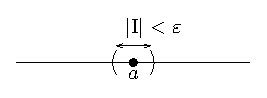
\includegraphics[width=0.25\textwidth]{24_2.eps}
	\label{24_2}
	\caption{Множество меры ноль: точка.}
	\label{fig:Множество меры ноль}
\end{figure}
$2)$ \textbf{Конечный набор точек}: накроем точки $x_1,\dotsc, x_N$ интервалами $\MI_i$, длины которых меньше $\tfrac{\VE}{N}$. Таким образом, суммарная длина всех отрезков будет меньше $\VE$ и все интервалы покрывают весь конечный набор точек.
\begin{figure}[H]
	\centering
	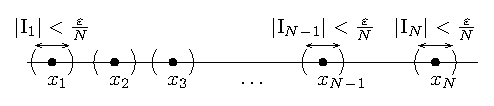
\includegraphics[width=0.55\textwidth]{24_3.eps}
	\label{24_3}
	\caption{Множество меры ноль: конечный набор точек.}
	\label{fig:Множество меры ноль}
\end{figure}
$3)$ \textbf{Счетный набор точек}: $\{x_n\}_{n=1}^{\infty}$ накрываем интервалами $\MI_i$, длина которых становятся меньше с ростом $n$. Например, интервалами длина которых меньше, чем $\dfrac{\VE}{2^{n+1}}$. Тогда:
$$
	\sum\limits_{n = 1}^{\infty}|\MI_n| < \VE \sum\limits_{n = 1}^{\infty}\dfrac{1}{2^{n+1}} = \VE
$$
$4)$ \textbf{Множество Кантора}: Отрезок $[0,1]$ делится на $3$ равные части, середина исключается. Потом оставшиеся интервалы снова делятся на $3$ равные части и середина снова исключается, и так далее. То, что останется будет множеством меры ноль. Сумма длин этих отрезков равна:
$$
	1 - \sum\limits_{n=1}^N\dfrac{2^{n-1}}{3^n}\to 0
$$
Это значит, что на каждом шаге можно оставшееся множество накрыть конечным числом отрезков, сумма длин которых будет меньше любого наперед заданного $\VE > 0$. Любой такой отрезок можно будет чуть-чуть расширить, чтобы получился интервал.

$5)$ \textbf{Отрезок}: Отрезок $[a,b]$ (где $b > a$) не является множеством меры ноль, поскольку сумму длин покрывающих интервалов сделать меньше, чем длина отрезка не получится. Об этом говорит следующая лемма.

\begin{lemma}
	Если $[a,b] \subset \displaystyle \bigcup\limits_n \MI_n$, где $\MI_n$ - интервалы, то верно следующее: 
	$$
		b - a \leq \displaystyle \sum\limits_n |\MI_n \cap [a,b]| \leq \displaystyle \sum\limits_n |\MI_n|
	$$	
\end{lemma}
\begin{rem}
	Из этой леммы следует еще одно доказательство того, что отрезок не является счетным множеством. Если бы он являлся счетным множеством, то был бы множеством меры ноль.
\end{rem}
\begin{proof}
	Отрезок это компакт, поэтому достаточно рассмотреть конечное покрытие. Пусть $[a,b] \subset \displaystyle \bigcup\limits_{n=1}^N \MI_n$. Будем доказывать индукцией по количеству интервалов	$N$.
	
	\textbf{\uline{База}}: $N = 1 \Rightarrow [a,b] \subset (\alpha,\beta) \Rightarrow b - a \leq |[a,b] \cap (\alpha,\beta)| = b-a  \leq \beta - \alpha$.
	
	\textbf{\uline{Шаг}}: Пусть верно для $N$, докажем для $N+1$. Можно считать, что $b \in \MI_{N+1} = (\alpha_{N+1}, \beta_{N+1})$. Пусть точка $\alpha_{N+1} \in [a,b]$, иначе смотри базу индукции. Рассмотрим отрезок $[a,\alpha_{N+1}]$, он целиком покрывается остальными интервалами:
	$$
		[a,\alpha_{N+1}] \subset \displaystyle \bigcup\limits_{n = 1}^{N} \MI_n
	$$
	Если это не так, то вместе с интервалом $(\alpha_{N+1}, \beta_{N+1})$ они бы не смогли покрыть отрезок $[a,b]$. Тогда:
	$$
		\alpha_{N+1} - a \leq \sum\limits_{n = 1}^{N} |[a,\alpha_{N+1}] \cap \MI_n|
	$$
	где верно следующее:
	$$
		\forall n, \, |[a,\alpha_{N+1}] \cap \MI_n| \leq |[a,b] \cap \MI_n|
	$$ 
	Добавим $b - \alpha_{N+1}$ к правой и левой части неравенства выше, получим:
	$$
		b - a \leq b - \alpha_{N+1} + \sum\limits_{n = 1}^{N} |[a,\alpha_{N+1}] \cap \MI_n| \leq b - \alpha_{N+1} + \sum\limits_{n = 1}^{N} |[a,b] \cap \MI_n| = |[a,b]\cap \MI_{N+1}| +  \sum\limits_{n = 1}^{N} |[a,b] \cap \MI_n|
	$$
	Учитывая, что $\forall n, \, |[a,b]\cap \MI_n| \leq |\MI_n|$ получим требуемое.
\end{proof}
\subsection*{Свойства множеств меры ноль}
$1)$ В определении множества меры ноль по Лебегу можно интервалы заменить отрезками.
\begin{proof}\hfill \\
	$(\Rightarrow)$ Если $\forall \VE > 0, \, \exists$ интервалы $\MI_n = (\alpha_n, \beta_n)$ такие, что: 
	$$
		E \subset \displaystyle \bigcup\limits_n \MI_n \wedge \sum\limits_{n}|\MI_n| < \VE
	$$ 
	то это выполнено и для отрезков $[\alpha_n,\beta_n]$. Поскольку $E$ содержится в объединении интервалов и их концов, а наличие или отсутствие точки  на сумму длин не сказыватеся. 
	
	$(\Leftarrow)$ Пусть теперь $\forall \VE > 0, \, \exists \, \MJ = [\alpha_n, \beta_n]$ такие, что:
	$$
		E \subset \bigcup\limits_n \MJ_n \wedge  \sum\limits_{n}|\MJ_n| < \VE
	$$
	Расширим отрезки до интервалов, увеличив длину в два раза:
	$$
		\MI_n = \left(\dfrac{\alpha_n + \beta_n}{2} - (\beta_n - \alpha_n),\dfrac{\alpha_n + \beta_n}{2} + (\beta_n - \alpha_n) \right), \, |\MI_n| = 2|\MJ_n| \Rightarrow  \sum\limits_{n}|\MI_n| < 2\VE
	$$
	А поскольку $\VE > 0$ - произвольное, то получим требуемое.
\end{proof}

$2)$ Если $E$ множество меры ноль и $D \subset E$, то $D$ - множество меры ноль.
\begin{proof}
	Очевидно, поскольку если смогли покрыть большее множество, то меньшее покроем тем более:
	$$
		D \subset E \subset \displaystyle \bigcup\limits_n \MI_n
	$$
	Сумма длин отрезков не меняется, следовательно получаем требуемое.
\end{proof}

$3)$ Если $E_n$ (не более, чем счетный набор) - множество меры ноль, то $\displaystyle \bigcup\limits_n E_n$ - множество меры ноль.
\begin{proof}
	По аналогии со счетным набором точек: каждое $E_n$ необходимо покрыть своим набором $\{\MI_k^n\}$ так, чтобы сумма их длин была меньше, чем $\dfrac{\VE}{2^{n+1}}$:
	$$
		E_n \subset \bigcup\limits_{k} \MI_k^n \wedge \sum\limits_{k}|\MI_k^n| < \dfrac{\VE}{2^{n+1}} \Rightarrow \bigcup\limits_n E_n \subset \bigcup\limits_{k,n} \MI_k^n \wedge \sum\limits_{k,n}|\MI_k^n| < \VE
	$$
	Таким образом, выполнено определение множества меры ноль.
\end{proof}
\begin{rem}
	Здесь стоит задаться вопросом, как мы смогли так просуммировать произвольно ряд по индексам $k,n$. У нас есть числа $a_k^n$ - длины отрезков $\MI_k^n$. Мы знаем, что сумма по $k$ при фиксированном $n$ меньше, чем $\dfrac{\VE}{2^{n+1}}$:
	$$
		\sum\limits_{k}a_k^n < \dfrac{\VE}{2^{n+1}}
	$$
	А теперь мы начинаем складывать по $k,n$: делаем нумерацию пар $(k,n)$ (например, по табличке или по диагонали, главное чтобы вся таблица была занумерована). Таким образом, мы получаем сопоставление: $j \rightarrow \left(k(j),n(j)\right)$ и строим сумму по $j$:
	$$
		\sum\limits_j a_{k(j)}^{n(j)}
	$$
	Именно это подразумевается, когда пишем сумму ряда по индексам $k,n \colon \displaystyle \sum\limits_{k,n}|\MI_k^n| < \VE$. Эта сумма есть предел частичных сумм:
	$$
		\sum\limits_j a_{k(j)}^{n(j)} = \lim\limits_{M \to \infty}\sum\limits_{j = 1}^M a_{k(j)}^{n(j)}
	$$
	В этой конечной сумме уже можно перераспределить слагаемые так, как будет удобно, например, по принадлежности к $n$: отдельно те, которые относятся к $1$ (если нет таких, то считаем слагаемое равным $0$), отдельно те, которые относятся к $2$ и так далее. Получим следующую сумму:
	$$
		\sum\limits_{j = 1}^M a_{k(j)}^{n(j)} = \sum\limits_{p} a_{p}^{1} + \sum\limits_{p} a_{p}^{2} + \dotsc + \sum\limits_{p} a_{p}^{M}  < \dfrac{\VE}{4} + \dfrac{\VE}{8} + \dotsc + \dfrac{\VE}{2^{M+1}}  < \VE
	$$
	Каждая частичная сумму меньше, чем $\VE \Rightarrow$ их предел меньше или равен $\VE$:
	$$
		\sum\limits_{k,n}|\MI_k^n| = \sum\limits_j a_{k(j)}^{n(j)} = \lim\limits_{M \to \infty}\sum\limits_{j = 1}^M a_{k(j)}^{n(j)} \leq \VE
	$$
\end{rem}
\section*{Критерий Лебега}
\begin{defn}
	Если некоторое свойство имеет место для всех точек, кроме множества меры ноль, то говорят, что это \uwave{свойство выполняется почти всюду}.
\end{defn}
\begin{theorem}(\textbf{Критерий Лебега})
	$f$ - интегрируема по Риману на отрезке $[a,b] \Leftrightarrow f$ - ограничена на отрезке $[a,b]$ и $f$ почти всюду непрерывна на отрезке $[a,b]$.
\end{theorem}
\begin{rem}
	Проще говоря, функция интегрируема тогда и только тогда, когда функция ограничена, а множество точек разрыва является множеством меры ноль по Лебегу.
\end{rem}

\end{document}